\documentclass{article}
\usepackage[utf8]{inputenc}
\usepackage[french]{babel}
\usepackage[T1]{fontenc}
\usepackage{fullpage}
\usepackage{graphicx}
\usepackage{subfig}
\usepackage{hyperref}

\begin{document}

\begin{titlepage}

\begin{center}
\newcommand{\HRule}{\rule{\linewidth}{0.5mm}}

\vspace{1cm}
\textsc{\LARGE INGInious}
\vspace{7cm}

\HRule \\[1cm]
{\huge \bfseries Création d'exercices sur INGInious\\ \vspace{0.4cm} Tutoriel\\[1cm]}
\HRule \\
\vspace{1.5cm}

\large{\emph Auteur : }\\
\vspace{0.3cm}

\textsc{Oreins} Manon\\

\vfill


\large Juillet 2020
\end{center}
\end{titlepage}

\section{Créer et activer son compte}

Pour commencer, accédez au syllabus en ligne via le lien suivant :

\bigskip
\url{https://math-syllabus.info.ucl.ac.be}
\bigskip

Vous aurez alors accès à la table des matières et aux cartes conceptuelles. Cependant, les exercices vous serons inaccessibles tant que vous ne serez pas connecté. 

Cliquez donc sur "Log in" en haut à gauche de la page 

\begin{figure}[!htb]
    \centering
    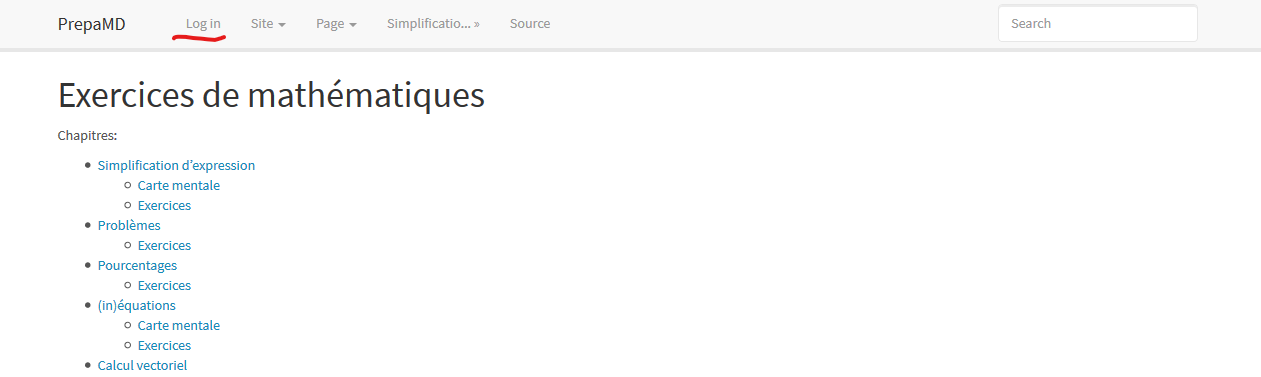
\includegraphics[scale=0.4]{images/login.png}
\end{figure}

Vous arriverez ensuite ici :

\begin{figure}[!htb]
    \centering
    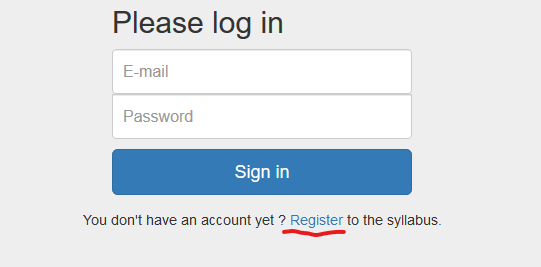
\includegraphics[scale=0.5]{images/register.png}
\end{figure}

Si vous possédez un compte, connectez-vous, sinon cliquez sur "Register". Inscrivez ensuite une adresse mail existante. Après validation, ceci devrait apparaitre

\begin{figure}[!htb]
    \centering
    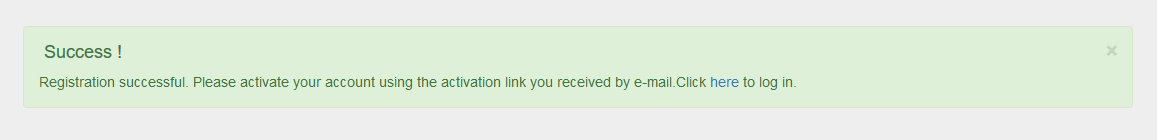
\includegraphics[scale=0.5]{images/mail.png}
\end{figure}

Rendez-vous donc sur votre boite mail où doit apparaitre un mail nommé "no-reply", vérifiez votre courrier indésirable s'il ne se trouve pas dans la boite de réception. Cliquez sur le lien du mail, vous devriez arriver sur une page affichant ceci :

\begin{figure}[!htb]
    \centering
    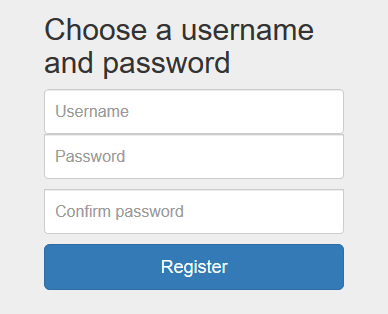
\includegraphics[scale=0.5]{images/choose_mdp.png}
\end{figure}

\newpage
Choisissez votre identifiant et votre mot de passe et cliquez sur "Register". Vous arrivez alors sur cette page :

\begin{figure}[!htb]
    \centering
    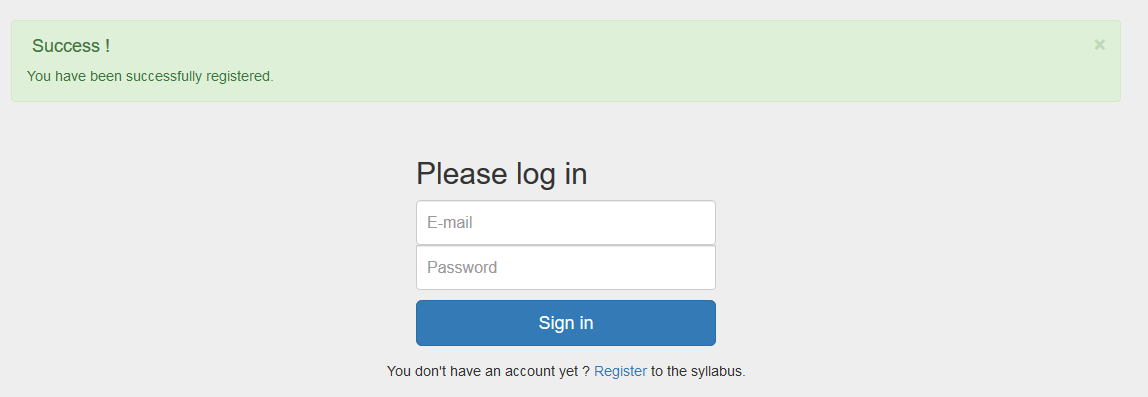
\includegraphics[scale=0.5]{images/Success.png}
\end{figure}

Votre compte est maintenant créé et activé. En vous connectant, utilisez votre adresse mail et non votre identifiant.

\section{Lier son compte à INGInious}

Vous avez maintenant normalement accès aux exercices présents dans le syllabus, cependant, ceci s'affiche à la place :

\begin{figure}[!htb]
    \centering
    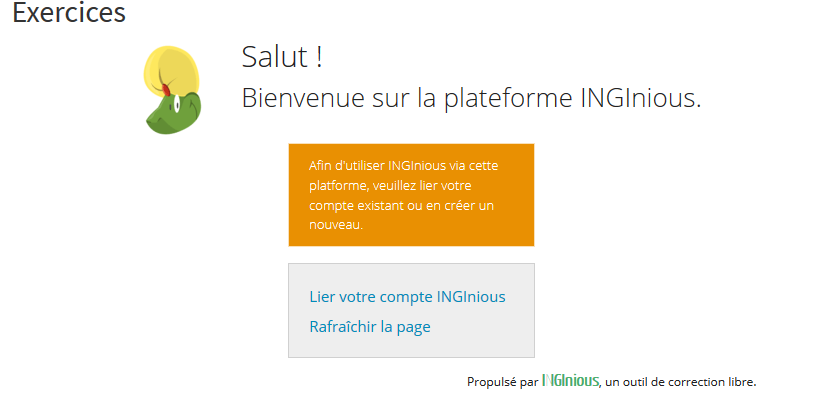
\includegraphics[scale=0.5]{images/Ingi.png}
\end{figure}

En effet, avant de pouvoir vous exercer, vous allez devoir lier un compte INGInious au compte que vous venez de créer.
Cliquez sur "Lier votre compte INGInious" de l'image précédente. Vous allez arriver ici :

\begin{figure}[!htb]
    \centering
    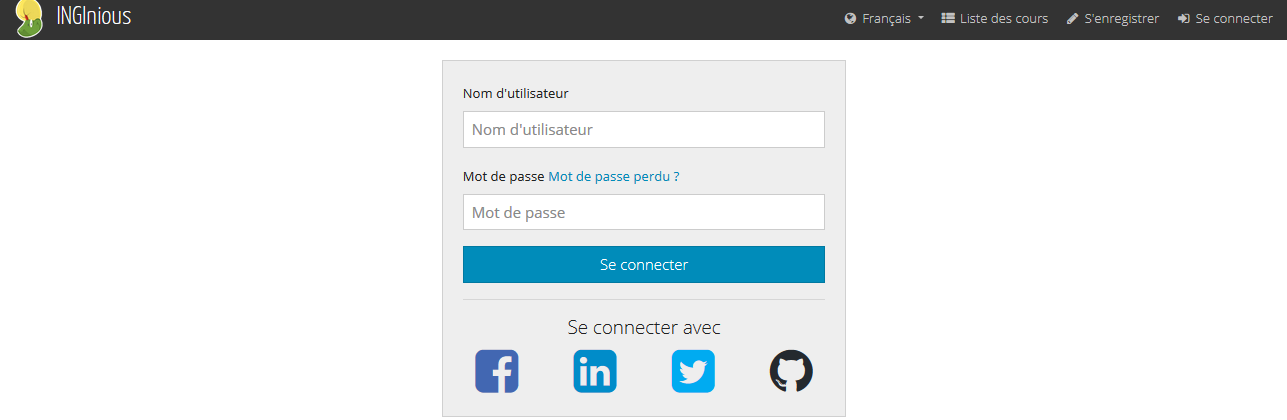
\includegraphics[scale=0.5]{images/inscription_INGI.png}
\end{figure}

Si vous possédez un compte, connectez-vous et suivez la procédure pour lier votre compte. Si vous n'en possédez pas, cliquez sur "S'enregistrer" en haut à droite. Vous allez être redirigé vers cette page :

\begin{figure}[!htb]
    \centering
    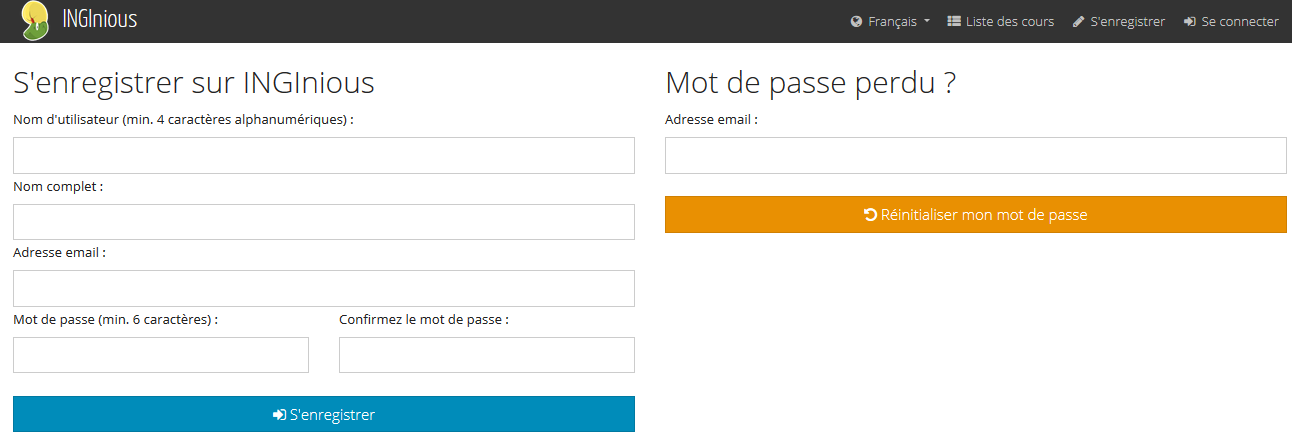
\includegraphics[scale=0.5]{images/enregistrement_INGI.png}
\end{figure}

Remplissez les différents champs et validez. Vous allez alors recevoir un mail, retrouvez-le dans votre boite et finalisez l'activation de votre compte INGInious. 

\bigskip
Une fois cela terminé, retournez sur le site du syllabus et cliquez une nouvelle fois sur "Lier votre compte INGInious". Vous arrivez alors sur une page intitulée "Liaison à un LMS existant", cliquez sur "Lier mon compte". 

\bigskip

Rafraîchissez la page et vous avez maintenant accès à tous les exercices du syllabus.














\end{document}
